\documentclass[tikz]{standalone}
\usepackage[utf8]{inputenc} 			
\usepackage[norsk]{babel}

\usepackage{amsmath, amssymb, amsthm, mathtools}   % Mijøer og verktøy for å
\usepackage{esdiff}
\let\div\relax
\DeclareMathOperator{\div}{div}
\DeclareMathOperator{\curl}{curl}
\DeclareMathOperator{\grad}{grad}
    
\newcommand{\vek}[1]{\mathbf{#1}}
\newcommand*{\dd}{\mathop{}\!{\operator@font d}}
\newcommand{\F}{\vek{F}}
\newcommand{\rr}{\vek{r}}
\newcommand{\dr}{\mathop{}\! \mathrm{d} \vek{r}\mathop{}\! }
\newcommand{\dt}{\mathop{}\! \mathrm{d} \vek{t}\mathop{}\! }
\newcommand{\dSS}{\mathop{}\! \mathrm{d} \vek{S}\mathop{}\! }

\newcommand{\R}{\mathbb{R}}

\usetikzlibrary{shapes.geometric, arrows}

\tikzstyle{startstop} = [rectangle, rounded corners, minimum width=3cm, minimum
height=1cm,text centered, draw=black, fill=red!30]
\tikzstyle{starting} = [trapezium, trapezium left angle=70, trapezium right
angle=110, rounded corners, minimum width=1cm, minimum
height=1cm,text centered, draw=black, fill=blue!40]
\tikzstyle{io} = [trapezium,
trapezium left angle=70, trapezium right angle=110, minimum width=3cm, minimum
height=1cm, text centered, draw=black, fill=blue!30]
\tikzstyle{process} =
[rectangle, minimum width=3cm, minimum height=1cm, text centered, draw=black,
fill=orange!30]
\tikzstyle{decision} = [diamond, minimum width=3cm, minimum
height=1cm, text centered, draw=black, fill=green!30]

\tikzstyle{arrow} = [thick,->,>=stealth]

\begin{document}

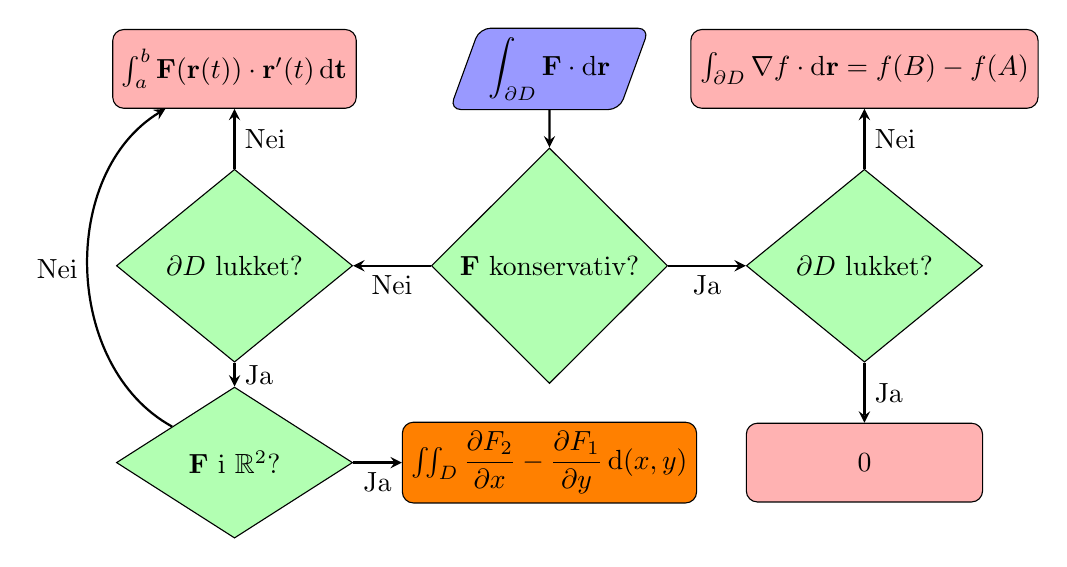
\begin{tikzpicture}[node distance=2cm]

  \node (start) [starting] {$\displaystyle \int_{\partial D} \F \cdot \dr$};
  \node (dec1) [decision, below of=start, yshift=-0.5cm, align=left] {$\F$ konservativ?};
  \node (dec2) [decision, right of=dec1, xshift=2cm] {$\partial D$ lukket?};
  \node (dec3) [decision, left of=dec1, xshift=-2cm] {$\partial D$ lukket?};
  \node (stop1) [startstop, below of=dec2, yshift=-0.5cm, align=left] {$0$};
  \node (stop2) [startstop, above of=dec2, yshift=0.5cm, align=left] {$\int_{\partial D} \nabla f \cdot \dr = f(B) - f(A)$};
  \node (stop3) [startstop, above of=dec3, yshift=0.5cm, align=left] {$\int_a^b \F(\rr(t)) \cdot \rr'(t) \dt$};
  \node (dec4) [decision, below of=dec3, yshift=-0.5cm] {$\F$ i $\R^2$?};
  \node (stop4) [startstop, fill=orange, below of=dec1, yshift=-0.5cm, align=left] {$\iint_{D} \diffp{{F_2}}{x} - \diffp{{F_1}}{y} \,\mathrm{d}(x,y)$};

  % \draw [arrow] (dec6) -- node[anchor=west] {Nei} (stop4);

  % \node (temp) [right of=dec5, xshift=2cm] {};

  \draw [arrow] (start) -- (dec1);
  \draw [arrow] (dec1) -- node[anchor=north] {Ja} (dec2);
  \draw [arrow] (dec3) -- node[anchor=west] {Ja} (dec4);
  \draw [arrow] (dec4) -- node[anchor=north] {Ja} (stop4);
  \draw [arrow] (dec2) -- node[anchor=west] {Ja} (stop1);
  \draw [arrow] (dec1) -- node[anchor=north] {Nei} (dec3);
  \draw [arrow] (dec3) -- node[anchor=west] {Nei} (stop3);
  \draw [arrow] (dec2) -- node[anchor=west] {Nei} (stop2);
  \draw [arrow] (dec4)  to [bend left=60] node[midway,left] {Nei} (stop3);
  
  % \draw [arrow] (dec2) -- node[anchor=west] {Ja} (stop1);
\end{tikzpicture}

\end{document}